\clearpage
\section*{2026-09-16: Parcel identity and full development coverage}
\textit{Agent-drafted research entry; updated after the Flatbush filing-site check.}

The 1,198-square-foot input for 90 Flatbush Avenue is the area of a small old
lot, not the later 441-unit tower site. Official records identify a
12,603-square-foot replacement tower parcel. DOB's displayed application names
three original lots whose earlier recorded areas sum to 16,531 square feet.
The broader zoning site is 61,399 square feet. Distinguishing these land
boundaries is necessary before revising the model's site characteristics.

\textit{Correction to the initial results.} The first map comparison reported
27 whole-parcel matches, 102 partial-parcel sites, 32 missing later maps,
three earlier-coverage gaps, and two mixed-vintage parents. It overlooked
condominium polygons drawn under billing identifiers because it searched only
for their physical base lots. Using the filing BBL when mapped, then a
physical base or a unique mapped condominium alias, recovers all 19 historical
parents in the missing-map group. Four become whole-parcel matches and fifteen
become partial-parcel comparisons. The current counts are \textbf{31 whole,
117 partial, 13 missing later maps, three earlier-coverage gaps, and two
mixed-vintage parents}. All 13 missing later maps concern post-policy parents.
The audit still covers 120 historical and 46 post-policy parents; the two
mixed-vintage parents retain both observations, giving 168 comparison rows.

Nine of the 31 whole-parcel matches retain another source/date flag. Tightening
the two-sided area tolerance from 2\% to 1\% or 0.5\% leaves 25 matches, eight
with additional flags. Among the 117 partial sites, the median earlier-union
area outside the later filing parcels is 45.5\%; 51 have more than half outside.
The spatial calculation identifies the overlapping old parcels without
assuming that every entire ancestor parcel belongs to the residential parent.

\subsection*{Flatbush establishes that the same lot number can change meaning}

The reference map, 18v2\_1, records old lots 18, 23, and 24 at 12,240, 1,198,
and 3,093 square feet, respectively. Their sum is 16,531. The corrected spatial
intersection independently identifies these three lots, exactly matching the
original tax-lot list displayed for DOB job 321595145. Their mapped union is
about 17,980 square feet; the later tower polygon is about 12,802. Recorded
areas and polygon areas remain separate measurements.

DOF merger 88954 on February 12, 2020 combines lots 9, 11, 13, 18, 23, and 24
into lot 13. Apportionment 88955 that morning divides the result into lots 13
and 23. Thus lot 23 was dropped and recreated with a different boundary.
The 2008 and 2020 dated tax maps visibly establish the change. A subsequent
2021 condominium declaration connects the tower base lot to its condominium
records; MapPLUTO 25v4 draws the footprint under billing lot 7502.

NYCIDA's May 12, 2020 board minutes, PDF page 41, independently distinguish
the 12,603-square-foot residential tower site from a 26,981-square-foot school
site; page 49 identifies them as block 174, lots 23 and 13. DOB's current
application displays a larger shared zoning site, with lots 1, 7, 10, 13,
and 23 and an area of 61,399. Giving that full zoning area to this one
residential parent would require a defensible allocation of the shared site.
The current DOB fields may include amendments. The original zoning drawing's
viewer did not expose the scan, so its boundary allocation remains unverified.

\subsection*{Dated maps and original filing lots provide systematic checks}

The earlier closest-map exercise is retained for its original 32-parent
physical-base cohort. Searching 23 saved 2018--2023 releases finds complete
base-ID maps for 18 historical parents within 3--100 days of first filing,
one post-policy parent 648 days before filing, and none for the other thirteen.
All 19 archived matches have later physical DOF transactions involving those
identifiers. The updated output saves those transactions and requires dated
tracing before treating an old number as the later boundary. This supersedes
the earlier interpretation of seven aligned maps as boundary confirmation.
Transactions are checked through the frozen September 15, 2026 snapshot;
some postdate 25v4 and do not establish which changes that map incorporated.

A targeted browser capture adds DOB site fields for 17 filings representing
14 historical parents. Eleven parents have positive reference-map areas for
all listed original parcels: nine sums exceed production and two equal it.
Three remain incomplete. Seven original-lot sets agree exactly with the
material spatial overlaps. At 2686 Broadway, the three original lots total
10,789 square feet versus 3,531 in production. At 46--10 70 Street, DOB names
original lots 41, 44, and 50, totaling 40,407 versus 305 in production, while
the spatial comparison also includes part of old lot 9. These differences
identify scope questions; they are not automatically adopted corrections.

Suffolk and Norfolk display the same original and zoning lot lists. Their
original parcels total 51,879 square feet, while the displayed zoning area is
51,884. Assigning either full shared-site measure separately to both parents
would duplicate land. Original parcels are counted once within each reviewed
parent; shared zoning lists are flagged without changing parent membership.
Missing lots at Snediker and Village Lane, and Bay Street's blank original-lot
field, remain missing. Subsequent BIS page access was denied, and the original
filed site diagrams were not verified.

Production land characteristics, constituent and parent panels, and calibration
files remain unchanged. The next substantive requirement is consistent full
filing-site coverage through dated DOF changes, including land shared across
phases or parents. The thirteen missing later-map cases are not an automatic
manual-research list. Neither a primary BBL, all its historical ancestors,
nor the whole zoning site alone establishes the model's pre-existing land.

\textit{Reproduction.} Working changes based on revision \texttt{a665b53}; run
\texttt{make dof-geometry-review}. The existing parcel audit owns the 166-parent
geometry comparison, its 168-page atlas, the 32-parent dated-map exercise,
and \path{bis_filing_sites.csv}/\path{bis_parent_site_comparison.csv}.
The acquisition task's \path{filing_sites_2026-09-16/README.md} records source
URLs, document pages, hashes, and browser-transcription limits. No new task
or main-pipeline dependency is introduced. SaveData writes the data reports.

\begin{figure}[p]
\centering
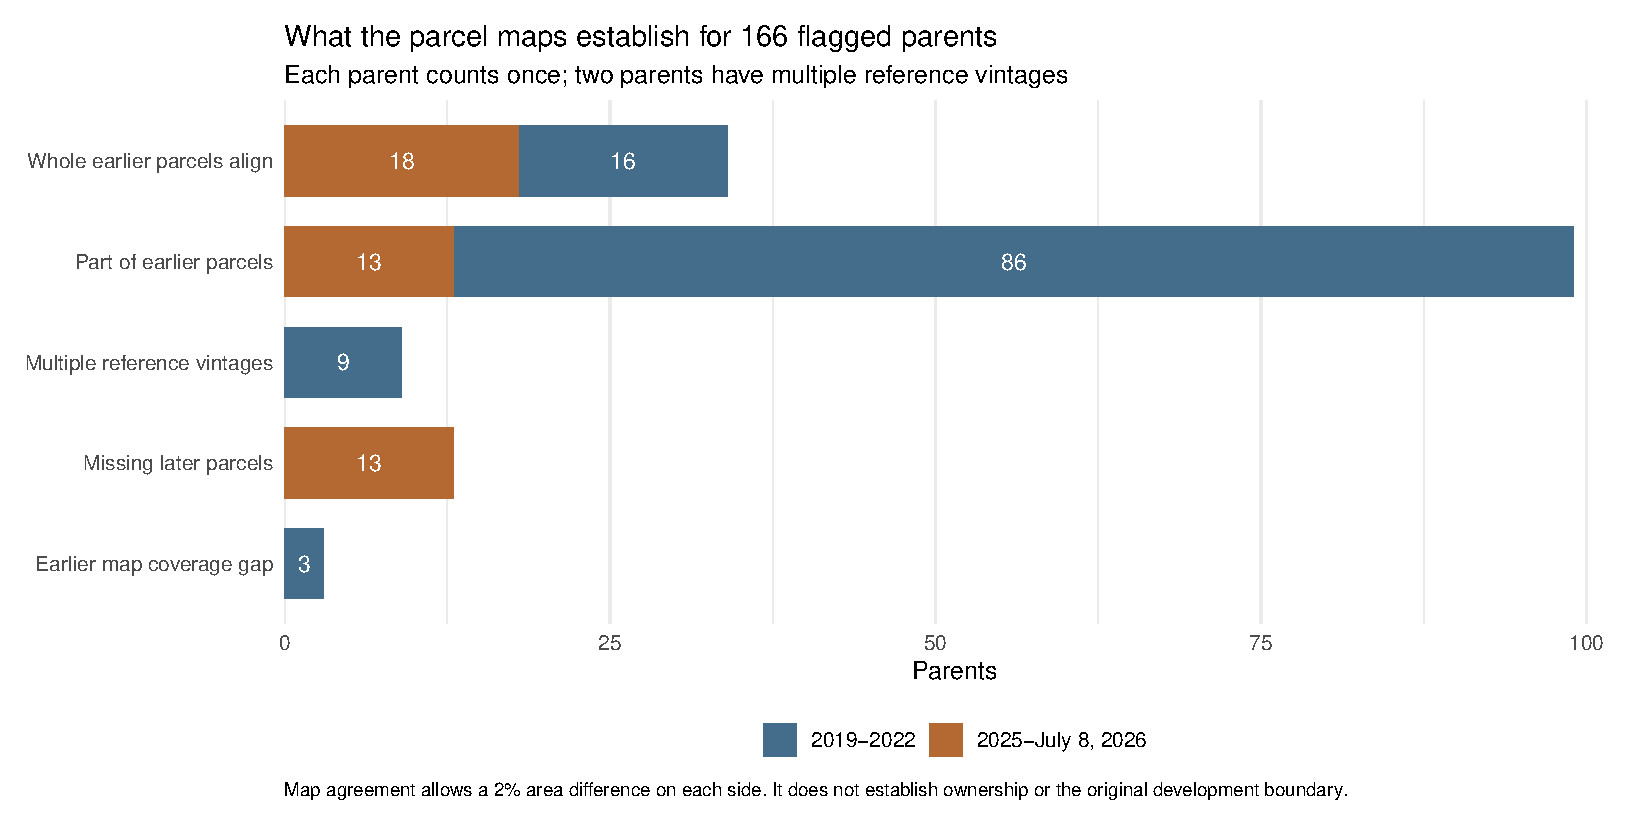
\includegraphics[width=\textwidth]{figures/dof_geometry_overview.pdf}
\caption{Corrected map comparisons for the 166 flagged parents, including
condominium billing polygons. Each parent counts once. Parcel alignment
establishes geographic agreement, not the developer's entire original site.}
\end{figure}
